\documentclass[20pt,landscape,dvips]{foils} 
% add 'draft' option above to exclude image when compiling
\usepackage[french]{babel}
\usepackage[utf8]{inputenc}  
\usepackage[french=guillemets*]{csquotes} 
\MakeOuterQuote{"}
\frenchspacing
\DecimalMathComma

\usepackage{latexsym}
\usepackage{amsmath,amssymb,amsfonts}
\usepackage{MnSymbol}
\usepackage{url}
\usepackage{graphicx}
%\usepackage[dvipsnames]{xcolor}
\usepackage{hyperref}
\usepackage{alltt}
\usepackage{pifont,manfnt}
\usepackage[dvipsnames,table]{xcolor}
\usepackage{subfig}
%\usepackage{enumerate}
%\usepackage{colortbl}
\usepackage{multirow,hhline}
\usepackage{cclicenses}
\setlength\parindent{0pt}
\hypersetup{colorlinks=true,citecolor=black,urlcolor=black,linkcolor=black}
\usepackage[style=verbose]{biblatex}
\bibliography{refs}

\newcommand{\highlight}[1]{\textcolor{Plum}{\bfseries #1}}
\newcommand{\remark}[1]{%
%\centerline{
\begin{center}
\framebox[.9\textwidth][t]{
\ding{46} 
\parbox[t]{.8\textwidth}{\small #1}}
\end{center}}

\DeclareMathOperator*{\inlaw}{\sim}
\newcommand{\iid}{\inlaw_{\text{i.i.d.}}}
%\newcommand{\iid}{\mathop{\mathrm{diag}}}
\newcommand{\pobs}{p_{\text{obs}}}

\reversemarginpar
\def\mark{\marginpar{\dbend}}

%\newcommand{\bm}[1]{\mbox{\boldmath{$#1$}}}
\renewcommand{\abstractname}{Summary}
\newcommand\bs{\char '134}   %  a backslash character for the \tt font
%\renewcommand\refname{Additional Readings}

% customize header/footer
\rightheader{}
% Note about the copyleft symbol:
% I use a custom reversed and circled "c" char because \textcopyleft in
% the textcomp package does not support sans serif font.
% Also, "c" is shifted horizontally by 1ex to align with the circle.
%\Restriction{\mbox{\raisebox{1.5ex}{\rotatebox{180}{\textcircled{c\kern.1ex}}} 2009}, \url{www.aliquote.org}}
% now I use the CC licence...
% \Restriction{\cc 2016 \VCRevision}
\Restriction{\cc 2016 Module 11 EESPE}

\title{Méthodes psychométriques en qualité de vie}
\author{Christophe Lalanne\\EA 7334 REMES\\ Unité de Méthodologie des critères d’évaluation\\Université Paris-Diderot, Sorbonne Paris-Cité\\}
\date{
\includegraphics[height=18ex]{logo.eps}}

%%% This file has been generated by the vc bundle for TeX.
%%% Do not edit this file!
%%%
%%% Define Git specific macros.
\gdef\GITHash{f4328f7906d309e9224e3e5c2f7f36477f44e69f}%
\gdef\GITAbrHash{f4328f7}%
\gdef\GITParentHashes{136657e4877819e72dc9ebb2f209631a2a8d1057}%
\gdef\GITAbrParentHashes{136657e}%
\gdef\GITAuthorName{Christophe Lalanne}%
\gdef\GITAuthorEmail{ch.lalanne@gmail.com}%
\gdef\GITAuthorDate{2016-07-06 10:29:58 +0200}%
\gdef\GITCommitterName{Christophe Lalanne}%
\gdef\GITCommitterEmail{ch.lalanne@gmail.com}%
\gdef\GITCommitterDate{2016-07-06 10:29:58 +0200}%
%%% Define generic version control macros.
\gdef\VCRevision{\GITAbrHash}%
\gdef\VCAuthor{\GITAuthorName}%
\gdef\VCDateRAW{2016-07-06}%
\gdef\VCDateISO{2016-07-06}%
\gdef\VCDateTEX{2016/07/06}%
\gdef\VCTime{10:29:58 +0200}%
\gdef\VCModifiedText{\textcolor{red}{with local modifications!}}%
%%% Assume clean working copy.
\gdef\VCModified{0}%
\gdef\VCRevisionMod{\VCRevision}%


\begin{document}
\LogoOff
\maketitle
\rightfooter{\quad\textsf{\thepage}}


%---------------------------------------------------------------Slide-
\foilhead{}

\bigskip
{\centering 
\includegraphics[width=\textwidth]{figs/pain.eps}\par}


%---------------------------------------------------------------Slide-
\foilhead{Théorie classique des tests}
\begin{itemize}
\item Définition des mesures subjectives en santé, intérêt et enjeu.
\item Approche psychométrique de la mesure.
\item Propriétés d'un bon instrument de mesure (validité, fidélité de mesure).
\item Modèles de mesure, modèles à variables latentes.
\end{itemize}

\begin{quote}
  \highlight{Validation of instruments} is the process of determining
  whether there are grounds for believing that the instrument measures
  what it is intended to measure, and that it is useful for its
  intended purpose \autocite{Fayers2000}.
\end{quote}

% ---------------------------------------------------------------Slide-
\foilhead{Développement et validation d'un questionnaire}

{\centering 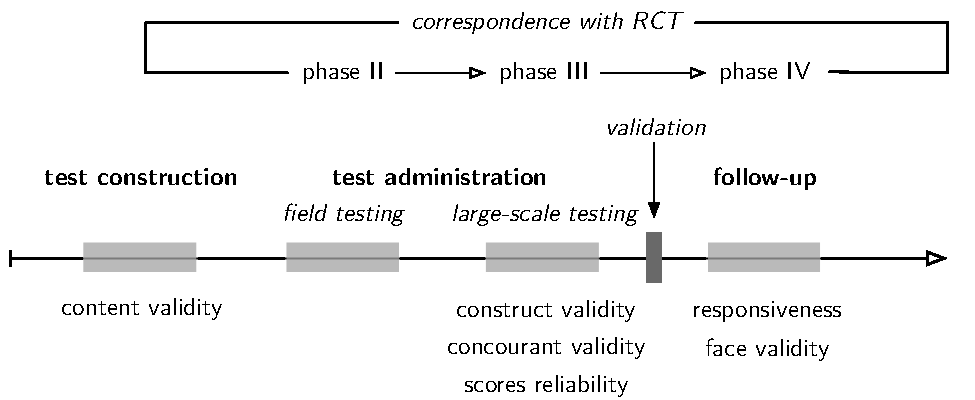
\includegraphics[width=.8\textwidth]{figs/testing.eps}\par}

%---------------------------------------------------------------Slide-
\foilhead{Taxonomie COSMIN\autocite{Mokkink2010}}

{\centering 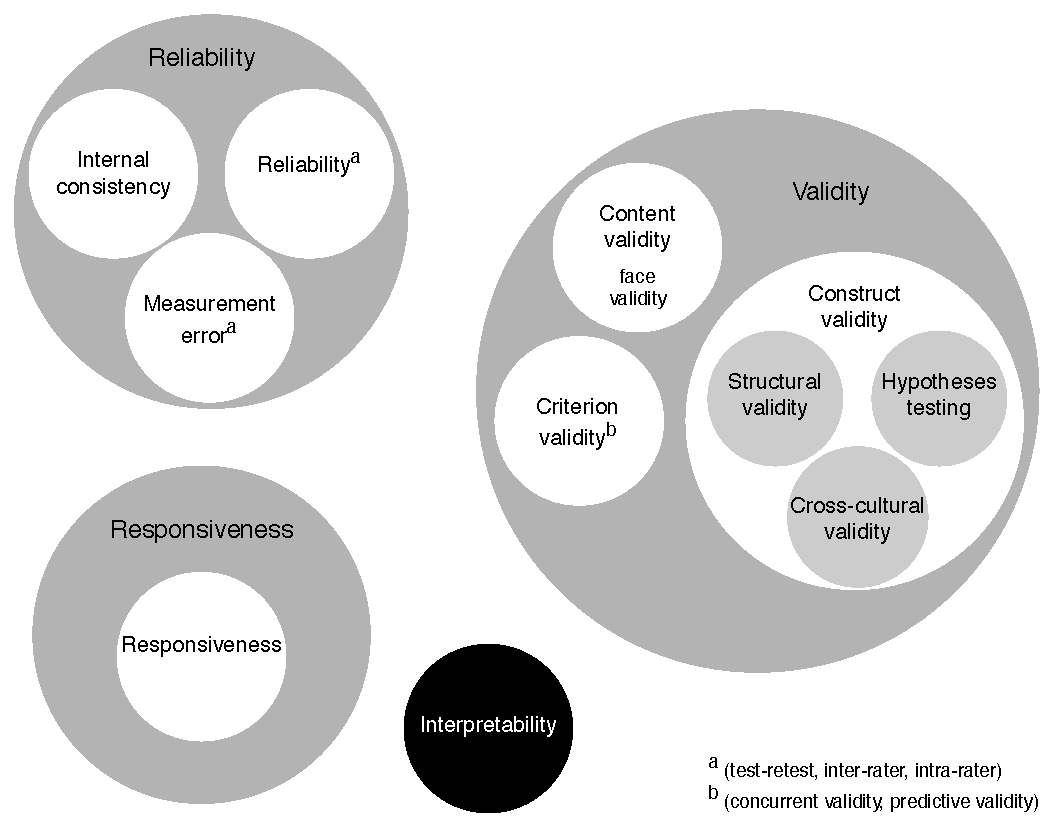
\includegraphics[width=.5\textwidth]{figs/cosmin_taxonomy.eps}\par}


%---------------------------------------------------------------Slide-
\foilhead{Instruments et mesures}

Un instrument est utilisé pour mettre en relation ou associer
\textcolor{Apricot}{quelque chose observé dans le monde réel} à
\textcolor{CornflowerBlue}{quelque chose de mesurable dans un certain cadre
  conceptuel}.

On parlera de \textcolor{Apricot}{variable manifeste} (p.ex., réponse à la
question "vous sentez-vous déprimé le matin en vous réveillant") et de
\textcolor{CornflowerBlue}{variable latente} (p.ex., "état dépressif" du
patient). 

On peut voir le processus de mesure comme une tâche consistant à assigner des
nombres à des catégories\autocite{Stevens1946,DeBoeck2005}.

%---------------------------------------------------------------Slide-
\foilhead{Construction d'un instrument de mesure\autocite{Wilson2005}}

\begin{itemize}
\item A \highlight{Construct map} features a coherent and substantive
  definition for the content of the construct which is composed of an
  underlying continuum (for ordering respondents and/or items
  responses).
\item \highlight{Items design} deals with the standardized
  construction of items that are supposed to stimulate responses,
  assimilable to observations about the construct. 
\item The \highlight{Outcome space} is the set of well-defined
  categories, finite and exhaustive, ordered, context-specific, and
  research-based.
\item A \highlight{Measurement model} is needed in order to relate the
  scored outcomes from the items design and the outcome space back to
  the construct that was the original inspiration of the items.
\end{itemize}


%---------------------------------------------------------------Slide-
\foilhead{Modèles à variables latentes}

La nature des variables manifestes et latentes permet généralement de guider le
choix d'un modèle statistique
\autocites{Bartholomew2011,RabeHesketh2008}.

\begin{center}\small
  \begin{tabular}{|c|c|c|c|}
    \cline{3-4}
    \multicolumn{2}{c|}{}&\multicolumn{2}{c|}{\textcolor{Apricot}{Variables manifestes}} \\
    \cline{3-4}
    \multicolumn{2}{c|}{}&\multicolumn{1}{c|}{Métrique} & \multicolumn{1}{c|}{Catégorielle} \\
    \hline
    \multirow{2}{*}{\textcolor{CornflowerBlue}{Variables latentes}} & Métrique & \highlight{Analyse factorielle} & \highlight{Analyse en traits latents} \\
    \cline{2-4}
    & Catégorielle & Analyse en profils latents & Analyse en classe latente\\
\hline
  \end{tabular}
\end{center}

% FIXME: rework this section

%---------------------------------------------------------------Slide-
\foilhead{Des items aux échelles de mesure}

Un \enquote{item} constitue l'unité de mesure fondamentale et il peut être
considéré comme une évaluation critériée d'un construit théorique
(\enquote{construct}) psychologique (fluence verbale, habileté cognitive,
qualité de vie, traits de personnalité).

L'aggrégation des réponses fournies par plusieurs individus à plusieurs items
permet de construire une échelle de mesure, souvent confondue avec la dimension
(construct) qu'elle est supposée refléter.

En supposant que cette échelle soit bel et bien unidimensionnelle, il est alors
possible d'assigner un score numérique aux patterns de réponse individuels et
ainsi positionner l'individu sur un trait latent.

%---------------------------------------------------------------Slide-
\foilhead{Illustration}

MOS 36-item version courte (1 =
\enquote{all the time},\ldots, 6 = \enquote{none of the time})

{\centering 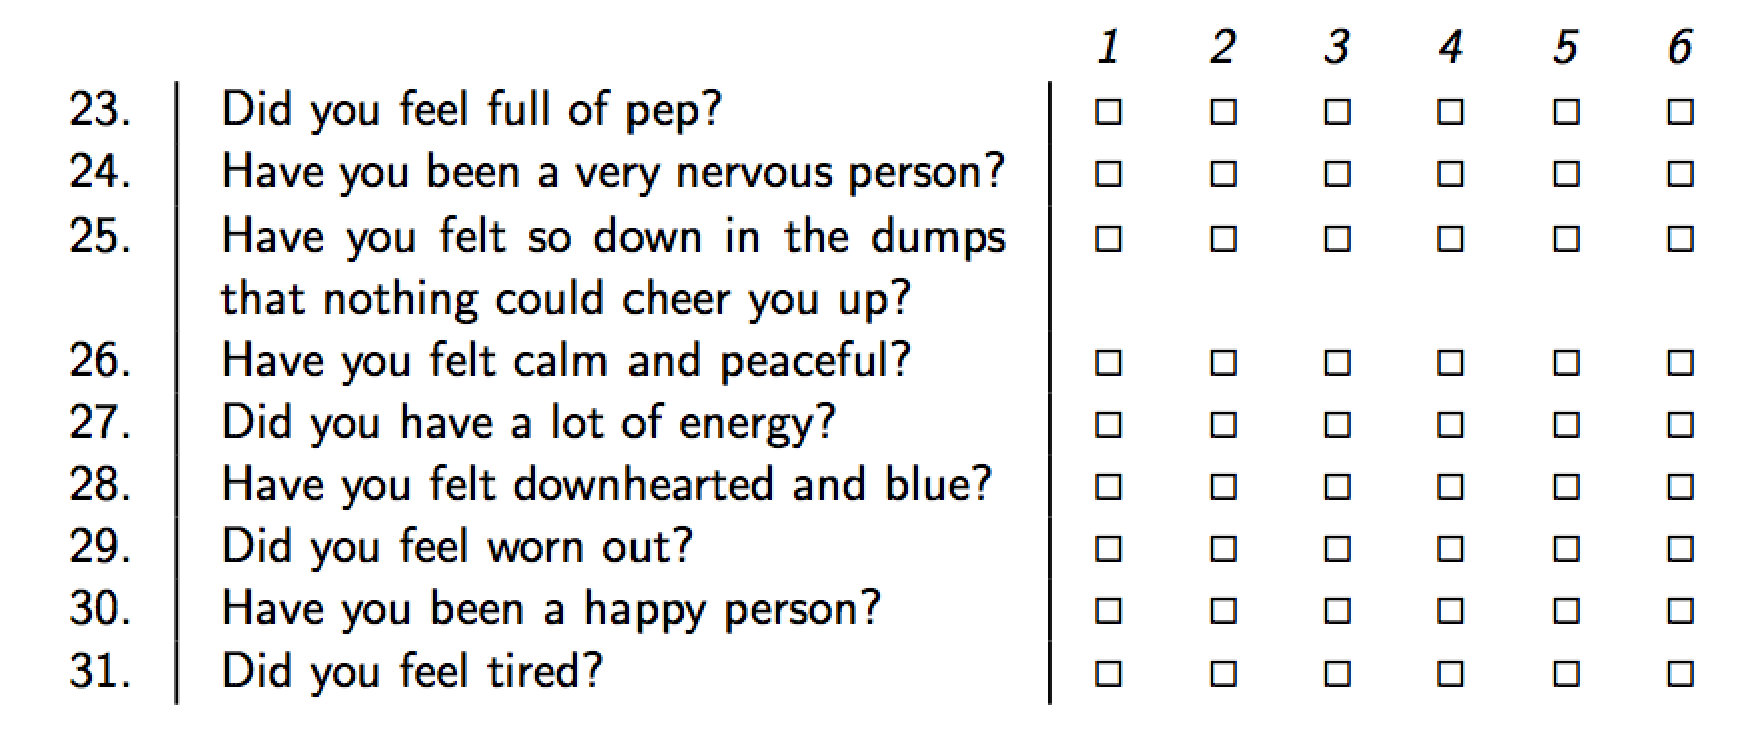
\includegraphics[width=.7\textwidth]{figs/mos_sf36.eps}\par}


%---------------------------------------------------------------Slide-
\foilhead{Type d'items}

\begin{itemize}
\item \highlight{item dichotomique} (variable binaire) : deux options de réponse
  ou plusieurs options de réponse mais une seule réponse correcte (p.ex., QCM) ;
\item \highlight{item polytomique} (variable catgéorielle ordinale) : options ou
  catégories de réponse naturellement ordonnées (p.ex., échelle de Likert)
\item score numérique (standardisé ou non) : application d'un algorithme pour
  dériver un score de résumé
\item choix préférentiels : choix ordonnés de réponses parmi un ensemble
  d'options de réponse
\end{itemize}

%---------------------------------------------------------------Slide-
\foilhead{Exemple d'échelles multidimensionnelles}

\begin{itemize}
\item Le questionnaire \highlight{HADS} est composé de deux dimensions ($2\times
  7$ items) permettant d'explorer les symptôme s
  anxio-dépressifs \autocite{Zigmond1983}.
\item Le \highlight{NEOPI-R} est un inventaire de personnalité (240 ou 60 items)
  basé sur le modèle en 5 facteurs (extraversion, agreeableness,
  conscientiousness, neuroticism, and openness; 6 facettes chacun)
  \autocite{McCrae1992}.
\item Le questionnaire \highlight{MOS-HIV} évalue la qualité de vie spécifique
  du VIH à l'aide de 35 items couvrant 10 dimensions suivantes\autocite{Wu1997a}.
\end{itemize}


%---------------------------------------------------------------Slide-
\foilhead{Propriétés attendues (en terme de mesure)}

\begin{itemize}
\item \highlight{unidimensionalité} : l'échelle de mesure mesure un seul
  construct qui est supposé expliquer les réponses d'un individu aux items selon
  sa position sur le trait latent ;
\item \highlight{indépendance locale} : si le trait latent est maintenu à une
  valeur constante, les réponses aux items sont indépendantes ;
\item \highlight{invariance de mesure} : les réponses individuelles ne dépendent
  pas de caratéristiques intrinsèques aux individus (p.ex., sexe, origine ethnique).
\end{itemize}

Les deux premières propriétés sont indispensables pour pouvoir attribuer un
score à l'individu (et aux items) sur le trait latent, tandis que la troisième
propriété permet des comparaisons inter-groupes valides.


%---------------------------------------------------------------Slide-
\foilhead{Les différentes facettes de la validité}

Plusieurs définitions ont été proposées sans grand concensus
\autocite{Falissard2008,Zumbo2007}.
\medskip

\begin{itemize}
\item \highlight{validité de contenu} : adéquation des domaines ou dimensions
  couvertes par les items ;
\item \highlight{validité de critère} : les échelles et donc les scores
  construits à partir d'elles ont des associations empiriques avec des critères
  externes (gold standard ou instruments mesurant des constructs similaires) ;
\item \highlight{validité de construit} (convergente et
  discriminante/divergente) : relation cohérentes des items et des
  sous-échelles entre elles.
\end{itemize}


% ---------------------------------------------------------------Slide-
\foilhead{Théorie classique des tests (TCT)}

Encore appelée \enquote{théorie du score vrai}, cette approche permet de
formaliser la construction d'un score permettant de caractériser un individu par
rapport à une échelle de mesure et de quantifier les sources potentielles de
variabilité ou d'erreur.

Le \textcolor{Apricot}{score} qui est assigné à un individu à partir de ses
réponses à un instrument de mesure standardisé (à un moment donné et dans des
conditions spécifiques) est ainsi envisagé comme une combinaison du
\textcolor{CornflowerBlue}{score vrai} et d'une \textcolor{Thistle}{erreur de
  mesure}.



%---------------------------------------------------------------Slide-
\foilhead{Modèle de mesure}

Pour un individu $i$ évalué sur une seule occasion, son score $x_i$ peut être
exprimé comme suit : 
\[
\textcolor{CornflowerBlue}{x_i} = \textcolor{Apricot}{\tau_i} +
\textcolor{Thistle}{\varepsilon_i}\, (i=1,\dots,n),\quad \varepsilon_i\sim\mathcal{N}(0;\sigma_e^2),
\]
d'où l'on en déduit naturellement que $\mathbb{E}(x)=\tau$.

Si l'on suppose que $T$ et $E$ sont indépendants, on a également
\[
\mathbb{V}(X) = \mathbb{V}(T)+\mathbb{V}(E).
\]

%---------------------------------------------------------------Slide-
\foilhead{Comment construire $X$}

Une façon simple de dériver un score résumant l'ensemble des réponses d'un
individu à un instrument comportant plusieurs items consiste à aggréger (par
sommation ou moyennage) l'ensemble des scores numériques associés à chaque item.

L'aggrégation peut être simple (non pondérée) mais il est également possible de
considérer une combinaison linéaire des scores aux items. Les poids de chaque
score peuvent être simples (coefficients entiers de pondération) ou plus
complexes (charges factorielles).

%---------------------------------------------------------------Slide-
\foilhead{Que trouve-ton dans $\varepsilon$}

L'erreur de mesure peut se décomposer en deux sources distinctes :
\begin{enumerate}
\item erreur systématique (ou biais), à éliminer au maximum dans la mesure du
  possible ; 
\item erreur aléatoire, propre à la variabilité intrinsèque de l'instrument de
  mesure. 
\end{enumerate}

Borsboom discute extensivement l'intérêt et les limitations d'une telle approche
pour la construction de scores, notamment la définition circulaire de la TCT \autocite{Borsboom2006,Borsboom2005}.



% %---------------------------------------------------------------Slide-
% \foilhead{Type de tests}

% On parle de \highlight{tests congénériquement équivalents} lorsque les tests
% peuvent être construits à partir d'un modèle unifactoriel et d'une erreur
% résiduelle. 

% \begin{itemize}
% \item Deux tests sont dits \highlight{parallèles} lorsque les charges
%   associées au modèle factoriel sont égales ($\lambda_1=\lambda_2$).
% \item Deux tests sont dits \highlight{tau-équivalents} lorsque les charges
%   factorielles sont égales mais que les erreurs diffèrent.
% \end{itemize}

% \vspace*{2em}
% \centerline{\includegraphics[scale=1]{figs/parallel_test.eps}}

% %---------------------------------------------------------------Slide-
% \foilhead{}

% Considérons les hypothèses suivantes :
% \begin{itemize}
% 	\item[($a_1$)] $\tau$-equivalence, $\tau_i=\tau_j$
% 	\item[($a_2$)] essential $\tau$-equivalence, $\tau_i = \tau_j + \lambda_{ij},\quad	\lambda_{ij} \in \mathbb{R}$
% 	\item[($a_3$)] $\tau$-congenerity, $\tau_i = \lambda_{ij0} + \lambda_{ij1}\tau_j,\quad	\lambda_{ij0}, \lambda_{ij1} \in  \mathbb{R}, \lambda_{ij1} > 0$
% \end{itemize}
% \begin{minipage}{0.6\textwidth}
% \begin{itemize}
% 	\item[($b$)] uncorrelated errors, $\text{cov}(\varepsilon_i,\varepsilon_j)=0, \forall i\neq j$
% 	\item[($c$)] equal error variances, $\mathbb{V}(\varepsilon_i)=\mathbb{V}(\varepsilon_j)$
% \end{itemize}
% \end{minipage}\hfill
% \begin{minipage}{0.35\textwidth}
% \centerline{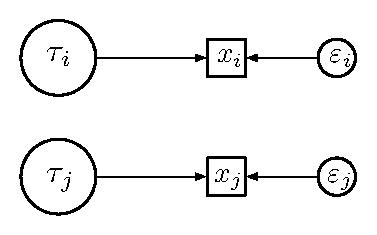
\includegraphics[scale=1]{figs/tau.eps}}
% \end{minipage}



%---------------------------------------------------------------Slide-
\foilhead{Illustration}

301 enfants de deux écoles auxquels on a administré 26 tests permettant d'évaluer les compétences suivantes : \textcolor{CornflowerBlue}{spatiales}, verbales, vitesse de raisonnement, mémoire, mathématiques.

\begin{quote}
  Holzinger, K. J. and Swineford, F. A. \emph{A study in factor analysis: The stability
  of a bi-factor solution}. Supplementary Education Monographs, 48. University of
  Chicago, 1939.  
\end{quote}

%---------------------------------------------------------------Slide-
\foilhead{}

{\centering \fbox{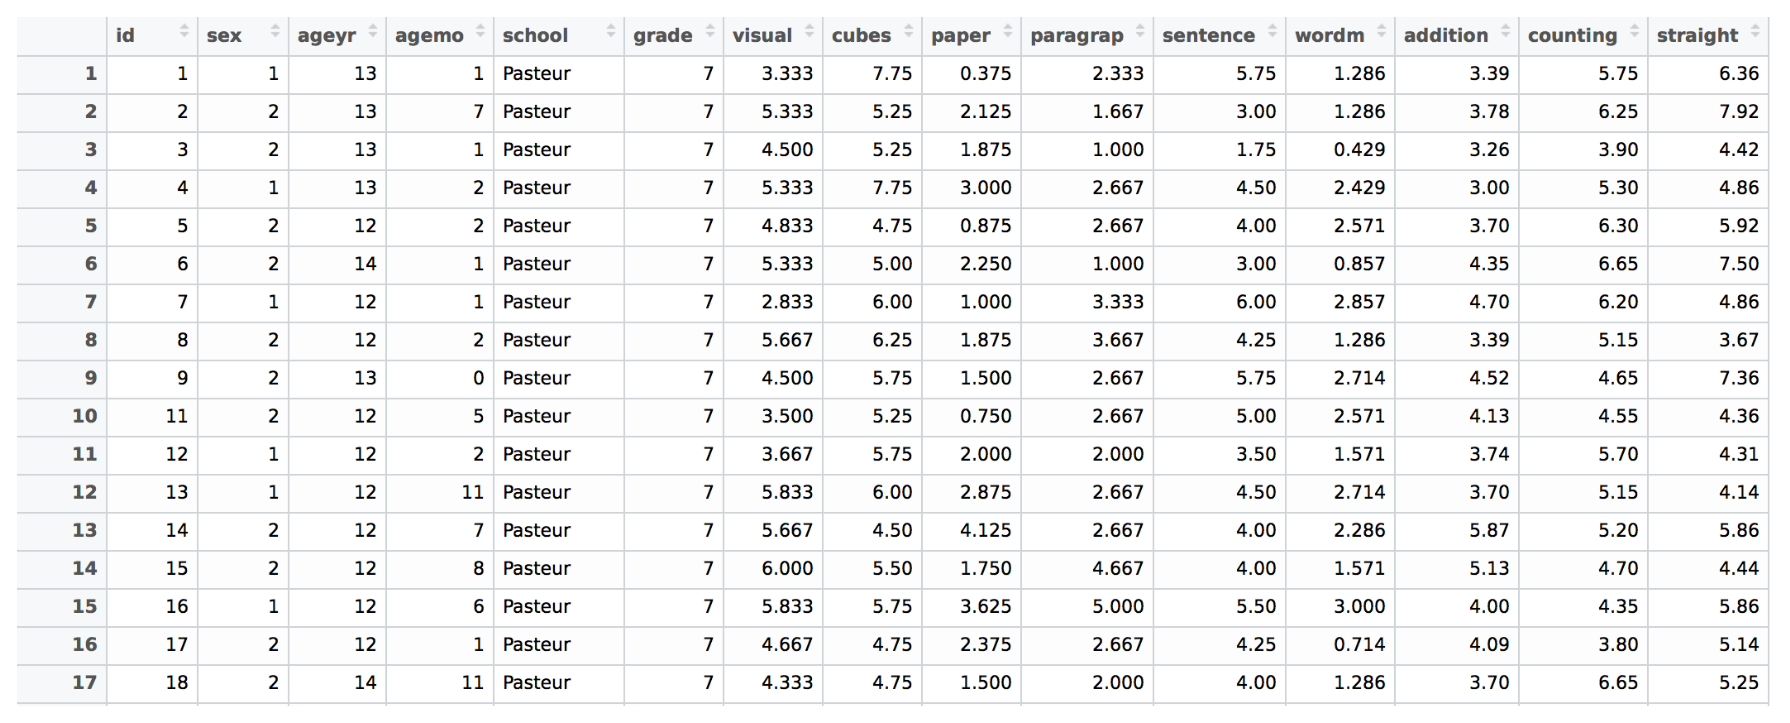
\includegraphics[width=.9\textwidth]{figs/HS.eps}}\par}


%---------------------------------------------------------------Slide-
\foilhead{Application avec R}

\begin{alltt}
data(HolzingerSwineford1939, package="lavaan") 
HS <- HolzingerSwineford1939
names(HS)[7:15] <- c("\textcolor{Apricot}{visual}", "\textcolor{Apricot}{cubes}", "\textcolor{Apricot}{paper}", \hfill\textcolor{CornflowerBlue}{\ding{182}}
                     "paragrap", "sentence", "wordm", \hfill\ding{183}
                     "addition", "counting", "straight") \hfill\ding{184}
\end{alltt}

\bigskip\bigskip

{\centering \textcolor{Apricot}{visual} + \textcolor{Apricot}{cubes} +
\textcolor{Apricot}{paper} = \textcolor{CornflowerBlue}{score (composite) spatial}\par}

%---------------------------------------------------------------Slide-
\foilhead{}

Calcul des scores composites :
\begin{alltt}
HS$spatial <- rowSums(HS[,c("visual","cubes","paper")])
HS$verbal <- rowSums(HS[,c("paragrap","sentence","wordm")])
HS$speed <- rowSums(HS[,c("addition","counting","straight")])
colMeans(HS[,c("spatial","verbal","speed")])
\end{alltt}
%$

% ---------------------------------------------------------------Slide-
\foilhead{}

{\centering 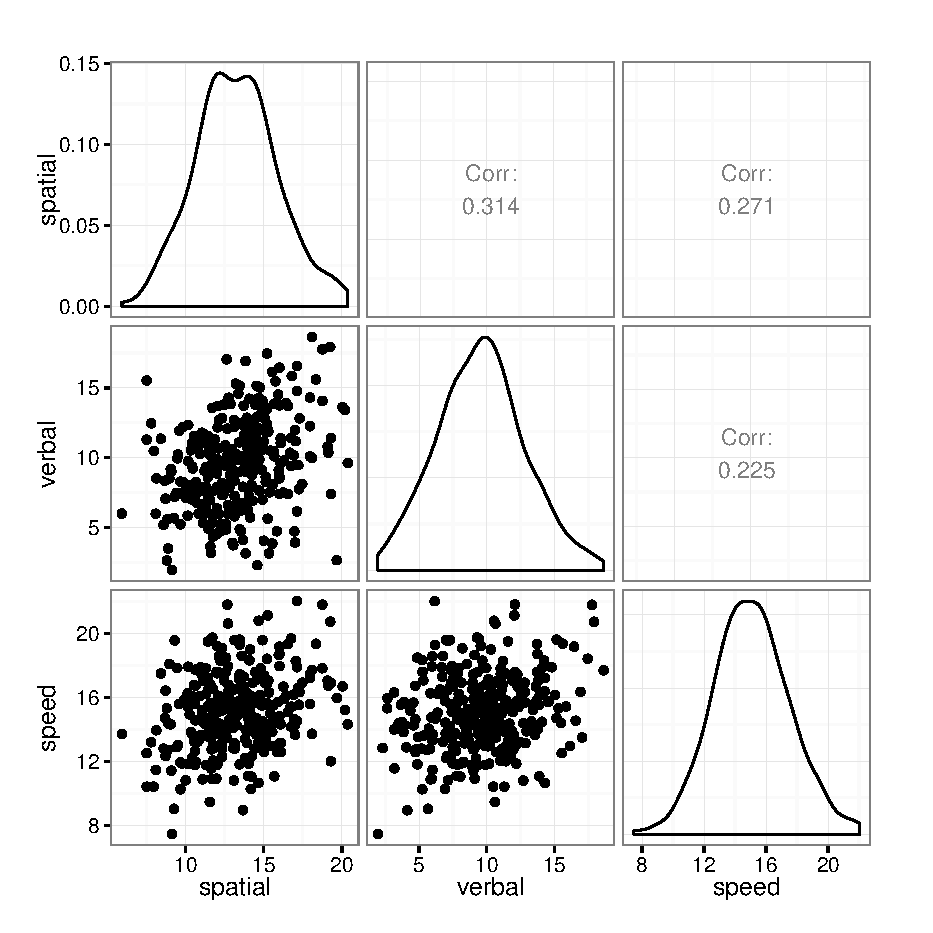
\includegraphics[width=.55\textwidth]{figs/fig-HS-ggpairs.eps}\par}

% ---------------------------------------------------------------Slide-
\foilhead{}

{\centering 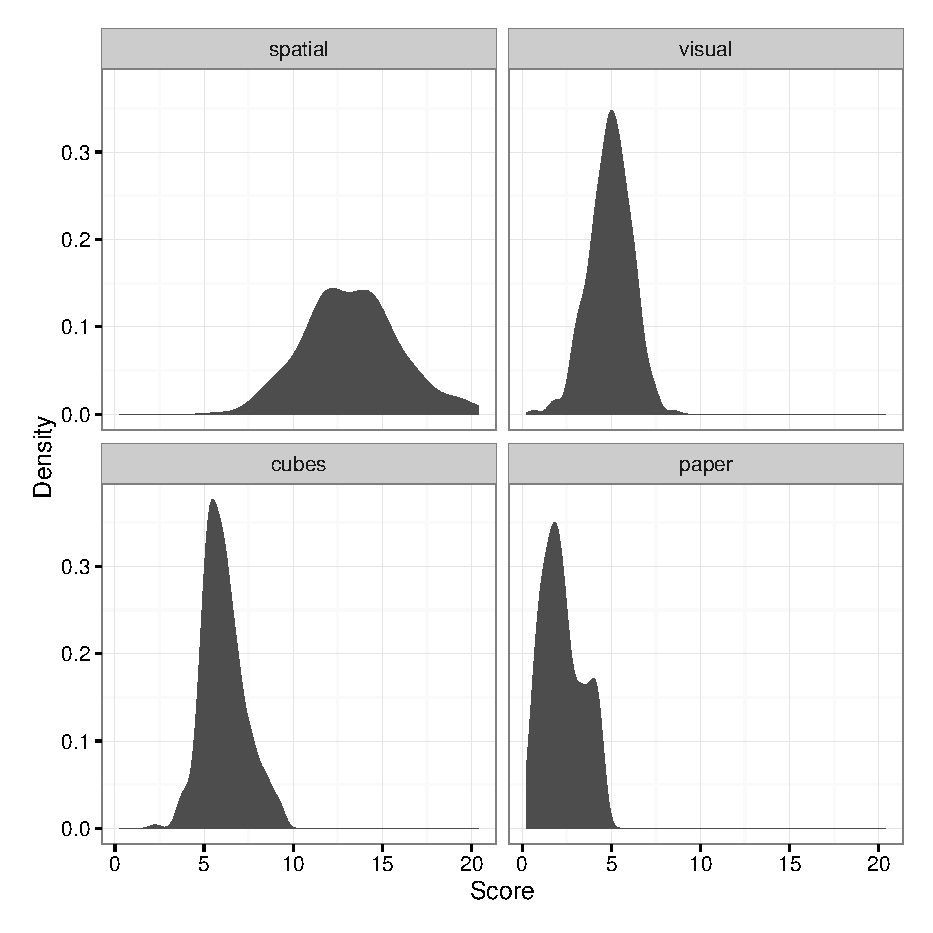
\includegraphics[width=.55\textwidth]{figs/fig-HS-hist.eps}\par}

% ---------------------------------------------------------------Slide-
\foilhead{Approche par ACP}

Les composantes $C_i$ ($i=1,\dots,p$) de l'analyse en composantes principales
(ACP) sont construites comme de simples combinaisons linéaires des $p$ variables
d'origine :
\[
C_i=\sum_{j=1}^pw_{ij}\textcolor{Apricot}{x_j}.
\]

Les charges $w_{ij}$ représentent la contribution de chaque variable dans la
composante $C_i$. Les valeurs propres représentent la part de variance expliquée
par chaque composante, et les vecteurs propres leur direction dans l'espace.

L'ACP constitue une approche préliminaire pour vérifier l'unidimensionnalité
d'une échelle de mesure.

% ---------------------------------------------------------------Slide-
\foilhead{}

{\centering 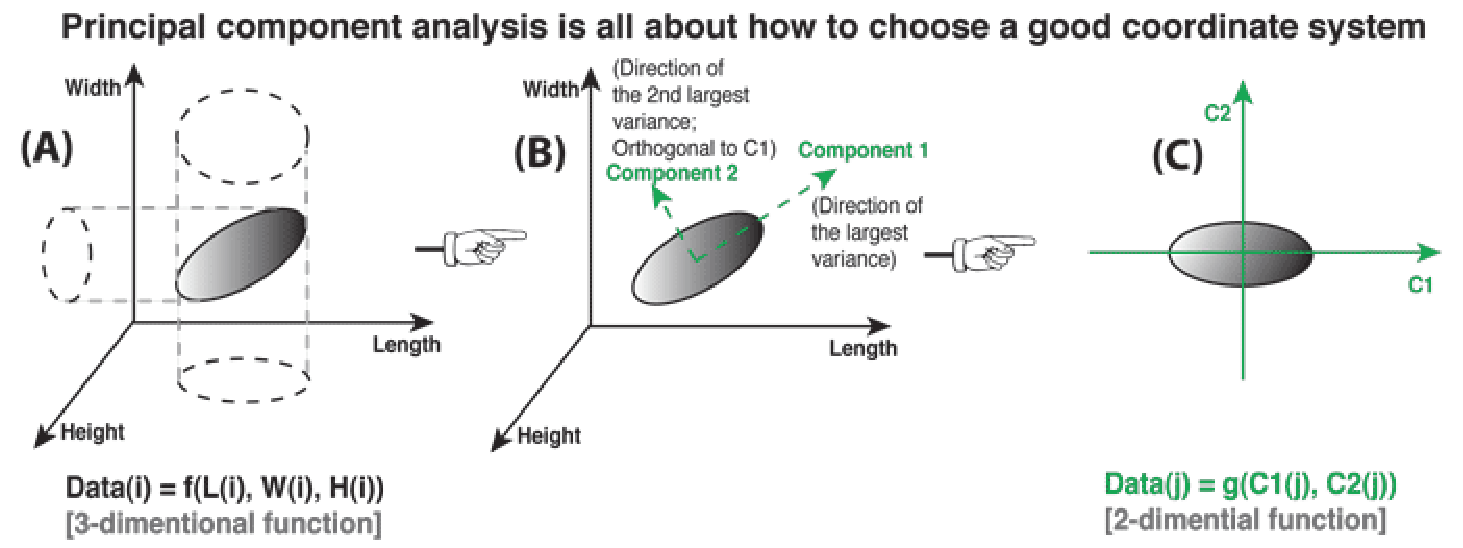
\includegraphics[width=.8\textwidth]{figs/fig-pca2.eps}\par}

\vfill
{\small Source : \url{http://mengnote.blogspot.fr/2013/05/an-intuitive-explanation-of-pca.html}}

% ---------------------------------------------------------------Slide-
\foilhead{Application pour l'échelle spatiale}


\begin{alltt}
library(FactoMineR)
pca <- PCA(HS[,c("visual", "cubes", "paper")], 
           scale.unit = TRUE, graph = FALSE)  
\end{alltt}
\begin{alltt}\small
> pca$eig
       eigenvalue percentage of variance cumulative percentage of variance
comp 1  1.7221050               57.40350                          57.40350  \ding{182}
comp 2  0.7227525               24.09175                          81.49525
comp 3  0.5551425               18.50475                         100.00000  
> pca$var
$coord
           Dim.1      Dim.2      Dim.3
visual 0.7742336 -0.4082765  0.4836038  \ding{183}
cubes  0.6951525  0.7115009  0.1026133
paper  0.7996439 -0.2232247 -0.5574409

$cor
           Dim.1      Dim.2      Dim.3
visual 0.7742336 -0.4082765  0.4836038  \ding{184}
cubes  0.6951525  0.7115009  0.1026133
paper  0.7996439 -0.2232247 -0.5574409

$cos2
           Dim.1      Dim.2     Dim.3
visual 0.5994377 0.16668969 0.2338726   \ding{185}
cubes  0.4832369 0.50623355 0.0105295
paper  0.6394303 0.04982925 0.3107404
\end{alltt}
%$

Packages R pour la visualisation des résultats : \texttt{ggbiplot},
\texttt{factoextra}.

Voir aussi : \url{http://gastonsanchez.com/how-to/2012/06/17/PCA-in-R/}.

% ---------------------------------------------------------------Slide-
\foilhead{}


{\centering 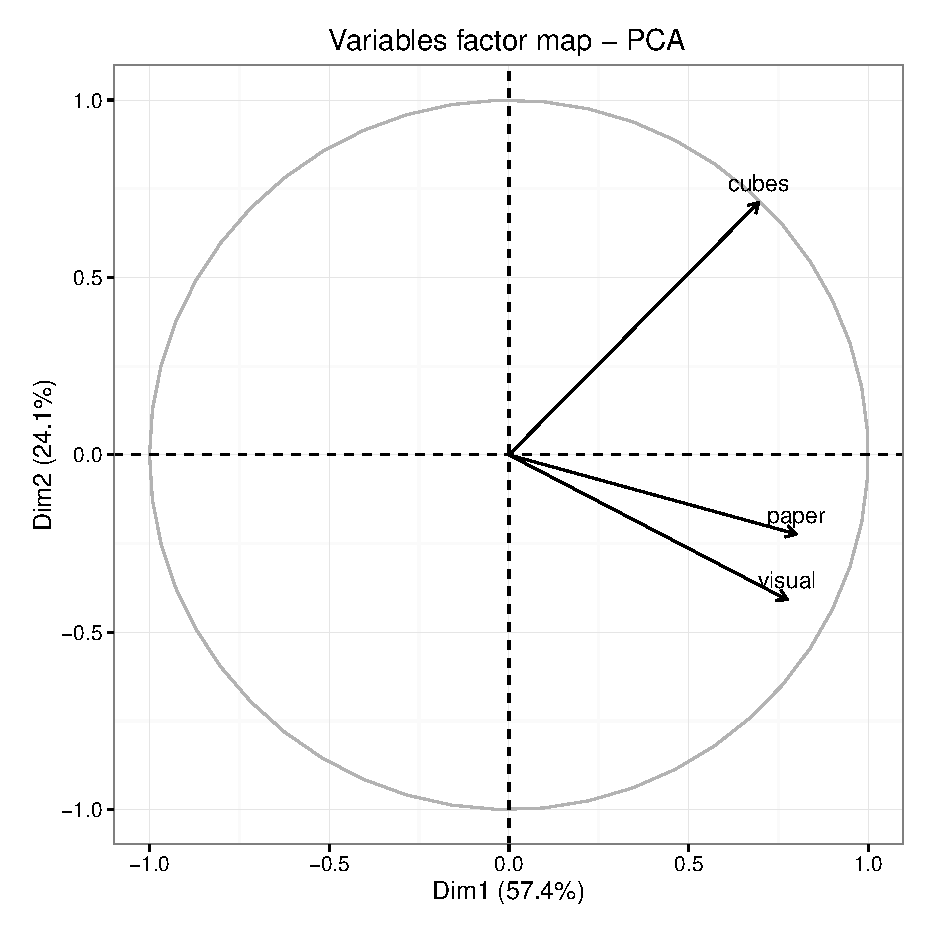
\includegraphics[width=.55\textwidth]{figs/fig-HS-pca.eps}\par}

% ---------------------------------------------------------------Slide-
\foilhead{Scores individuels}

{\centering \textcolor{Apricot}{visual} + \textcolor{Apricot}{cubes} +
\textcolor{Apricot}{paper} = \textcolor{CornflowerBlue}{score (composite) spatial}\par}

{\centering $w_{11}$\textcolor{Apricot}{visual} + $w_{12}$\textcolor{Apricot}{cubes} +
$w_{13}$\textcolor{Apricot}{paper} = PC1 $\approx$
\textcolor{CornflowerBlue}{score (factoriel) spatial}\par}

\begin{alltt}
HS$PC1 <- pca$ind$coord[,1]
cor(HS[,c("spatial","PC1")])  
\end{alltt}
%$

L'ACP peut être vue comme une méthode de réduction de dimension, de résumé
graphique d'une matrice de corrélation, voire d'inférence multivariée (sous
certaines hypothèses distributionnelles), mais dans tous les cas cette approche
suppose que les variables \textcolor{Apricot}{$X_j$} sont mesurées sans erreur.

Lorsque le nombe d'items est grand, l'ACP constitue une bonne approximation de
l'analyse factorielle.

% ---------------------------------------------------------------Slide-
\foilhead{Application}

\begin{enumerate}
\item Calculer la matrice de corrélation de Pearson et réaliser une ACP sur les
  données \texttt{HolzingerSwineford1939} en considérant l'ensemble des
  variables (\texttt{visual}, \ldots, \texttt{straight}).
\item Calculer les scores factoriels pour chaque dimension définie \emph{a
    priori} (3 variables/dimension) et calculer leur corrélation avec les scores
  totaux non pondérés.
\item Calculer les corrélations entre les sous-scores totaux et le score total
  calculé en ignorant les dimensions (9 variables).
\item Comparer les sous-scores totaux et factoriels entre les deux groupes de
  participants définis par la variable \texttt{school}.
\end{enumerate}


% ---------------------------------------------------------------Slide-
\foilhead{}

Fichier de données et scripts R disponibles à l'adresse suivante :\newline
{\centering \url{https://bitbucket.org/chlalanne/eespe11}\par}
\vfill

\raggedleft \scriptsize -- Typeset with \FoilTeX\ (version 2), Revision \VCRevision

\end{document}
